In this section we'll present a general overview of the system-to-be, with specific focus on the main logical components and their interactions.
The main high-level components of the system are:
\subsubsection{Mobile App:}
\label{subsubsect:Mobile App}
The presentation layer that let the users access the functionalities offered by the Travlendar+ on their smartphones. The mobile app offers also an internal logic that handle:
\begin{itemize}
\item notifications reception, through Google Cloud Messaging APIs;
\item map displaying and path drawing through Google Maps mobile APIs.
\end{itemize}  

\subsubsection{Web Browser:}
\label{subsubsect:Web Browser}
The presentation layer that let the users access the functionalities offered by the Travlendar+ on their browsers.
It relies on the connection with the web server in order to obtain dynamic web pages.
\subsubsection{Web server:}
\label{subsubsect:Web server}
This layer provide web pages for the web-based application, it communicate directly with the application server interfaces to satisfy the client requests, using proper Interfaces. This layer interact also with an external system (Google Maps API) in order to display an embedded map containing the user travel's information.

\subsubsection{Application Server:}
\label{subsubsect:Application Server}
The logic layer that implements all core system's functionalities. It receive and reply to client's requests, if required it send notifications to the mobile applications, it interact with external systems in order to satisfy the user's requests and it interact with a DBMS in order to guarantee the information persistence.
In particular the application server will interact with:
\begin{itemize}
\item Google Maps APIs in order to provide feasible paths according to the user preferences;
\item Transport Service providers systems to provide trips arranging functionalities, such as ticket buying, location of sharing vehicles and strikes informations.
\item Weather APIs in order to provide weather informations and to apply possible travel constraints related to the weather.
\item Google Cloud Messaging APIs ino order to send notifications to the user's mobile Apps.
\end{itemize} 
\subsubsection{Database Server:}
\label{subsubsect:Database Server}
The data layer, that supports all data storage and management operations. This layer ensure that ACID properties are satisfied. The database server will interact only with the application server, the data will never be exposed directly to the client layers.
\subsubsection{External Systems:}
\label{subsubsect:External Systems}
This are not internal components of our application, but the system-to-be will have to interact with them in order to guarantee all the system functionalities.
Most of their interactions with the system are already been described in the previous paragraphs, but here we'll explain in detail the interaction with Transport Service providers: Travlendar+ will initially integrate some external transport service systems (public transport service providers and sharing vehicles provider) but will also offer proper API to allow others Transport Service providers to interact with Travlendar+ and so to be considered as suggested travel means to the users.


\begin{figure}[H]
\begin{center}
		\hspace*{-50pt}
		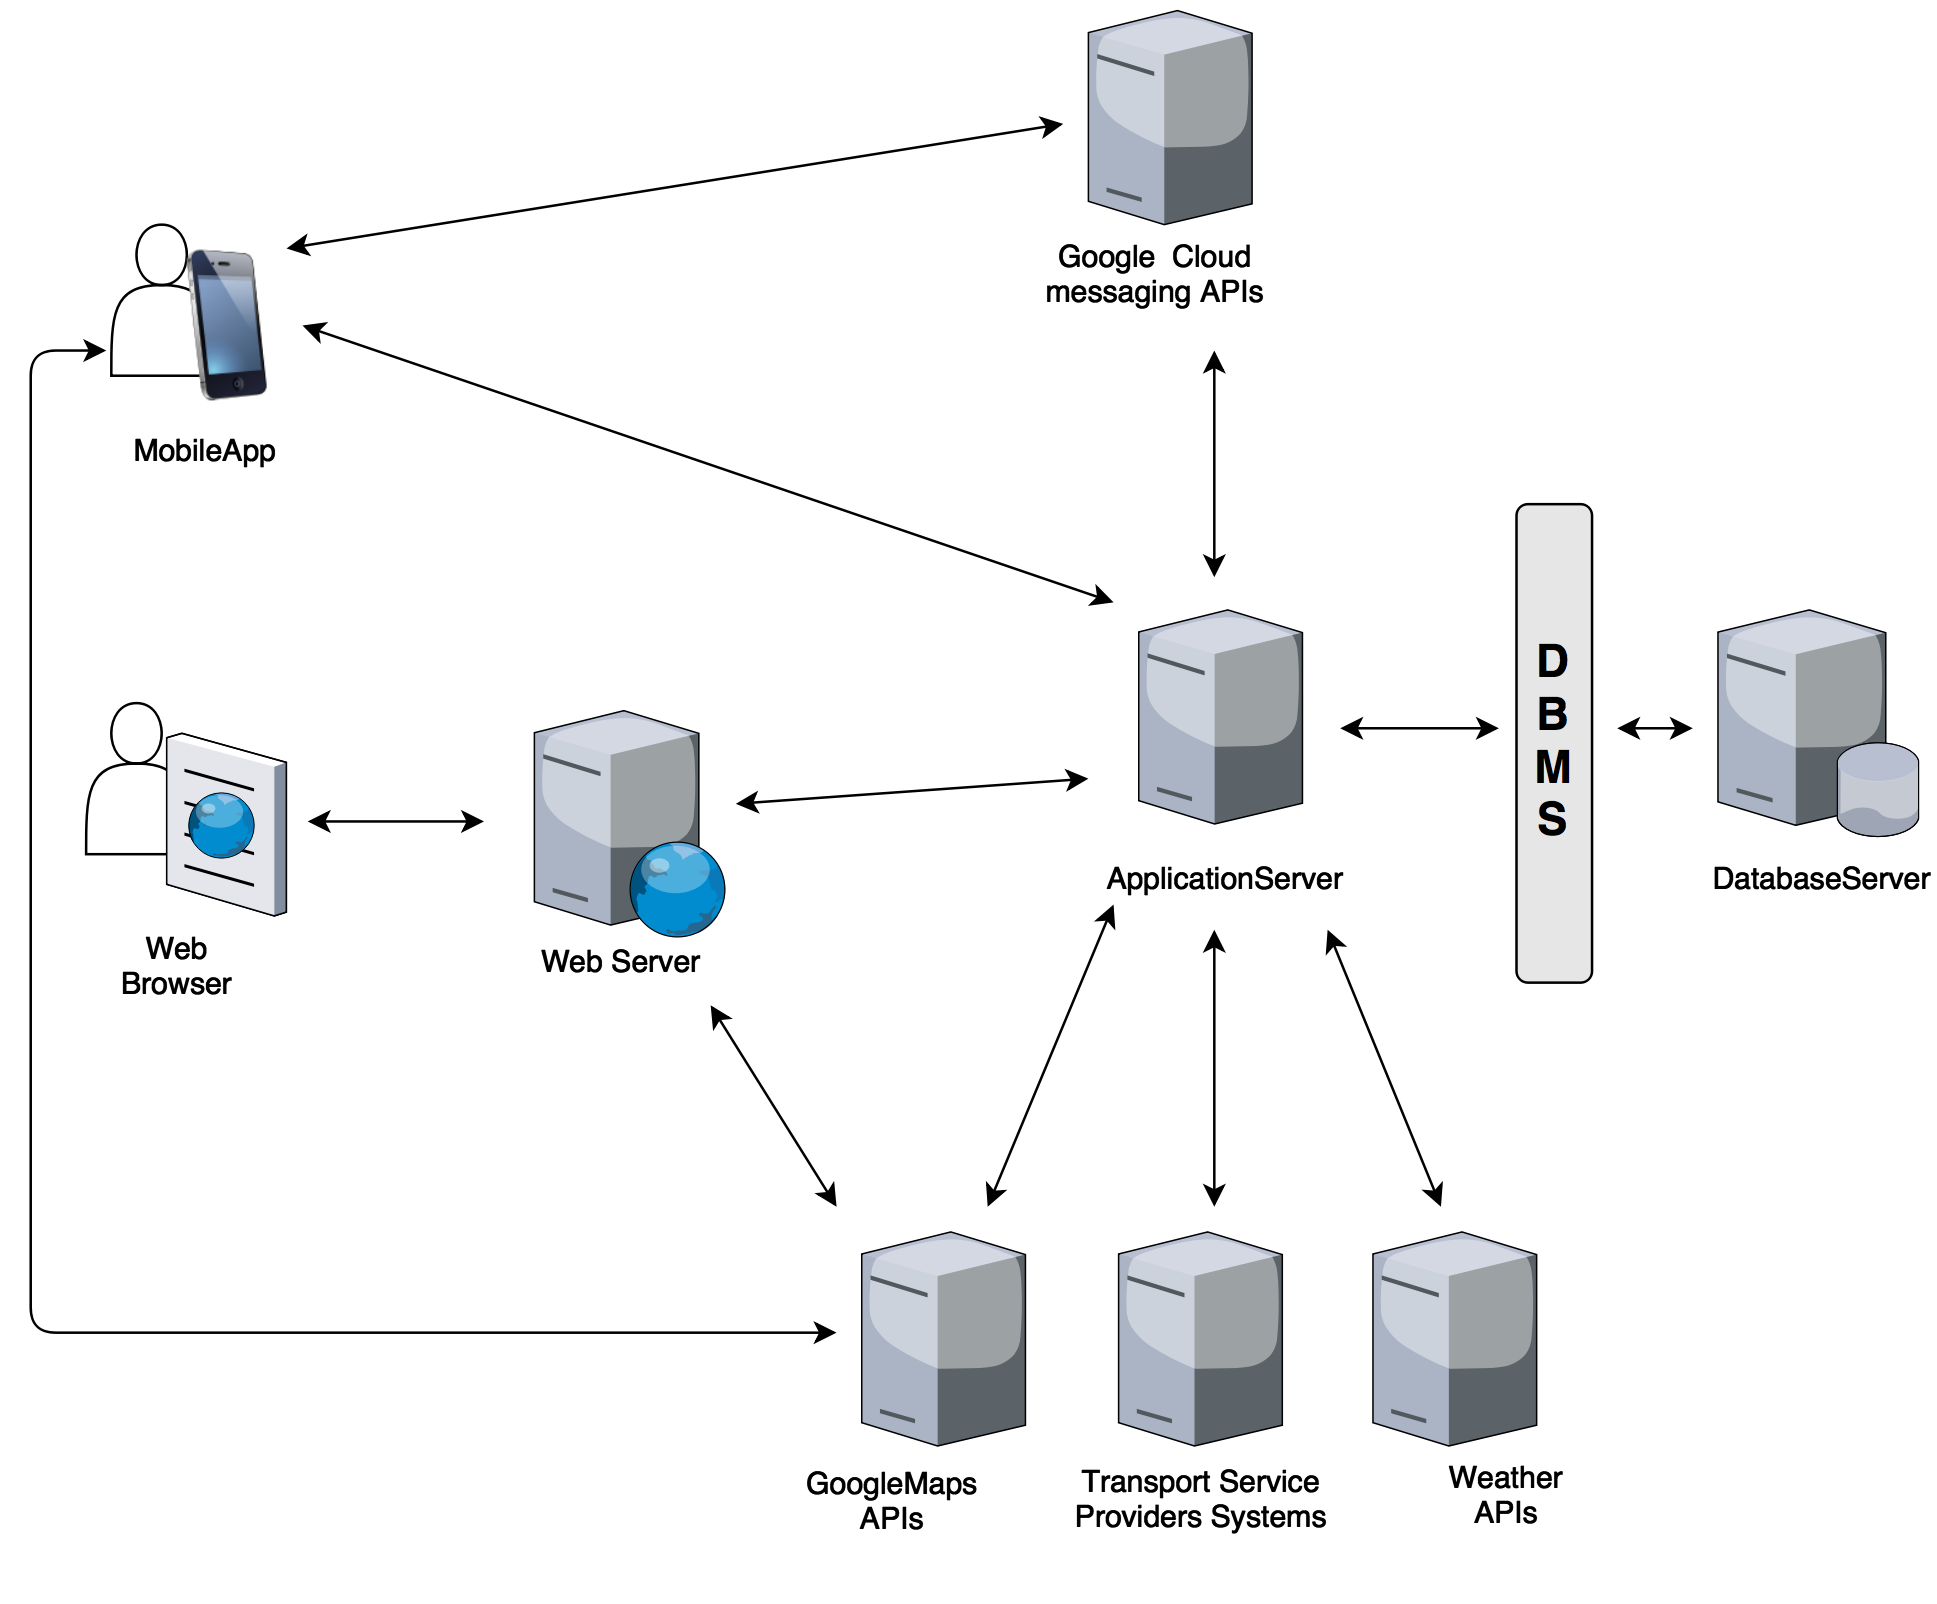
\includegraphics[scale=0.2]{GeneralArchitecture.png}
\end{center}
\caption{General Architecture}
\end{figure}
